\documentclass[twoside]{book}

% Packages required by doxygen
\usepackage{fixltx2e}
\usepackage{calc}
\usepackage{doxygen}
\usepackage[export]{adjustbox} % also loads graphicx
\usepackage{graphicx}
\usepackage[utf8]{inputenc}
\usepackage{makeidx}
\usepackage{multicol}
\usepackage{multirow}
\PassOptionsToPackage{warn}{textcomp}
\usepackage{textcomp}
\usepackage[nointegrals]{wasysym}
\usepackage[table]{xcolor}

% Font selection
\usepackage[T1]{fontenc}
\usepackage[scaled=.90]{helvet}
\usepackage{courier}
\usepackage{amssymb}
\usepackage{sectsty}
\renewcommand{\familydefault}{\sfdefault}
\allsectionsfont{%
  \fontseries{bc}\selectfont%
  \color{darkgray}%
}
\renewcommand{\DoxyLabelFont}{%
  \fontseries{bc}\selectfont%
  \color{darkgray}%
}
\newcommand{\+}{\discretionary{\mbox{\scriptsize$\hookleftarrow$}}{}{}}

% Page & text layout
\usepackage{geometry}
\geometry{%
  a4paper,%
  top=2.5cm,%
  bottom=2.5cm,%
  left=2.5cm,%
  right=2.5cm%
}
\tolerance=750
\hfuzz=15pt
\hbadness=750
\setlength{\emergencystretch}{15pt}
\setlength{\parindent}{0cm}
\setlength{\parskip}{3ex plus 2ex minus 2ex}
\makeatletter
\renewcommand{\paragraph}{%
  \@startsection{paragraph}{4}{0ex}{-1.0ex}{1.0ex}{%
    \normalfont\normalsize\bfseries\SS@parafont%
  }%
}
\renewcommand{\subparagraph}{%
  \@startsection{subparagraph}{5}{0ex}{-1.0ex}{1.0ex}{%
    \normalfont\normalsize\bfseries\SS@subparafont%
  }%
}
\makeatother

% Headers & footers
\usepackage{fancyhdr}
\pagestyle{fancyplain}
\fancyhead[LE]{\fancyplain{}{\bfseries\thepage}}
\fancyhead[CE]{\fancyplain{}{}}
\fancyhead[RE]{\fancyplain{}{\bfseries\leftmark}}
\fancyhead[LO]{\fancyplain{}{\bfseries\rightmark}}
\fancyhead[CO]{\fancyplain{}{}}
\fancyhead[RO]{\fancyplain{}{\bfseries\thepage}}
\fancyfoot[LE]{\fancyplain{}{}}
\fancyfoot[CE]{\fancyplain{}{}}
\fancyfoot[RE]{\fancyplain{}{\bfseries\scriptsize Generated by Doxygen }}
\fancyfoot[LO]{\fancyplain{}{\bfseries\scriptsize Generated by Doxygen }}
\fancyfoot[CO]{\fancyplain{}{}}
\fancyfoot[RO]{\fancyplain{}{}}
\renewcommand{\footrulewidth}{0.4pt}
\renewcommand{\chaptermark}[1]{%
  \markboth{#1}{}%
}
\renewcommand{\sectionmark}[1]{%
  \markright{\thesection\ #1}%
}

% Indices & bibliography
\usepackage{natbib}
\usepackage[titles]{tocloft}
\setcounter{tocdepth}{3}
\setcounter{secnumdepth}{5}
\makeindex

% Hyperlinks (required, but should be loaded last)
\usepackage{ifpdf}
\ifpdf
  \usepackage[pdftex,pagebackref=true]{hyperref}
\else
  \usepackage[ps2pdf,pagebackref=true]{hyperref}
\fi
\hypersetup{%
  colorlinks=true,%
  linkcolor=blue,%
  citecolor=blue,%
  unicode%
}

% Custom commands
\newcommand{\clearemptydoublepage}{%
  \newpage{\pagestyle{empty}\cleardoublepage}%
}

\usepackage{caption}
\captionsetup{labelsep=space,justification=centering,font={bf},singlelinecheck=off,skip=4pt,position=top}

%===== C O N T E N T S =====

\begin{document}

% Titlepage & ToC
\hypersetup{pageanchor=false,
             bookmarksnumbered=true,
             pdfencoding=unicode
            }
\pagenumbering{alph}
\begin{titlepage}
\vspace*{7cm}
\begin{center}%
{\Large Tribe\+Slot\+Cooldown Plugin }\\
\vspace*{1cm}
{\large Generated by Doxygen 1.8.14}\\
\end{center}
\end{titlepage}
\clearemptydoublepage
\pagenumbering{roman}
\tableofcontents
\clearemptydoublepage
\pagenumbering{arabic}
\hypersetup{pageanchor=true}

%--- Begin generated contents ---
\chapter{Namespace Index}
\section{Namespace List}
Here is a list of all namespaces with brief descriptions\+:\begin{DoxyCompactList}
\item\contentsline{section}{\mbox{\hyperlink{namespace_commands}{Commands}} }{\pageref{namespace_commands}}{}
\item\contentsline{section}{\mbox{\hyperlink{namespace_slot_cooldown}{Slot\+Cooldown}} }{\pageref{namespace_slot_cooldown}}{}
\end{DoxyCompactList}

\chapter{Class Index}
\section{Class List}
Here are the classes, structs, unions and interfaces with brief descriptions\+:\begin{DoxyCompactList}
\item\contentsline{section}{\mbox{\hyperlink{class_d_b_handler}{D\+B\+Handler}} }{\pageref{class_d_b_handler}}{}
\item\contentsline{section}{\mbox{\hyperlink{struct_commands_1_1_slot_cooldown__t}{Commands\+::\+Slot\+Cooldown\+\_\+t}} \\*Time struct }{\pageref{struct_commands_1_1_slot_cooldown__t}}{}
\end{DoxyCompactList}

\chapter{File Index}
\section{File List}
Here is a list of all files with brief descriptions\+:\begin{DoxyCompactList}
\item\contentsline{section}{Commands/\mbox{\hyperlink{_commands_8cpp}{Commands.\+cpp}} \\*Implementation of all \mbox{\hyperlink{namespace_commands}{Commands}} }{\pageref{_commands_8cpp}}{}
\item\contentsline{section}{Commands/\mbox{\hyperlink{_commands_8h}{Commands.\+h}} \\*Implementation of all \mbox{\hyperlink{namespace_commands}{Commands}} }{\pageref{_commands_8h}}{}
\item\contentsline{section}{D\+B\+Handler/\mbox{\hyperlink{_d_b_handler_8cpp}{D\+B\+Handler.\+cpp}} \\*Interface to the database }{\pageref{_d_b_handler_8cpp}}{}
\item\contentsline{section}{D\+B\+Handler/\mbox{\hyperlink{_d_b_handler_8h}{D\+B\+Handler.\+h}} \\*Interface to the database }{\pageref{_d_b_handler_8h}}{}
\item\contentsline{section}{Dll\+Main/\mbox{\hyperlink{_tribe_slot_cooldown_8cpp}{Tribe\+Slot\+Cooldown.\+cpp}} \\*Implementation of D\+L\+L\+Main }{\pageref{_tribe_slot_cooldown_8cpp}}{}
\item\contentsline{section}{Dll\+Main/\mbox{\hyperlink{_tribe_slot_cooldown_8h}{Tribe\+Slot\+Cooldown.\+h}} \\*Implementation of D\+L\+L\+Main }{\pageref{_tribe_slot_cooldown_8h}}{}
\item\contentsline{section}{Hooks/\mbox{\hyperlink{_hooks_8cpp}{Hooks.\+cpp}} \\*File containing the implementation for all needed Hooks }{\pageref{_hooks_8cpp}}{}
\item\contentsline{section}{Hooks/\mbox{\hyperlink{_hooks_8h}{Hooks.\+h}} \\*File containing the implementation for all needed Hooks }{\pageref{_hooks_8h}}{}
\item\contentsline{section}{Slot\+Cooldown/\mbox{\hyperlink{_slot_cooldown_8cpp}{Slot\+Cooldown.\+cpp}} \\*Implementation of the player slots cooldown logic }{\pageref{_slot_cooldown_8cpp}}{}
\item\contentsline{section}{Slot\+Cooldown/\mbox{\hyperlink{_slot_cooldown_8h}{Slot\+Cooldown.\+h}} \\*Implementation of the player slots cooldown logic }{\pageref{_slot_cooldown_8h}}{}
\end{DoxyCompactList}

\chapter{Namespace Documentation}
\hypertarget{namespace_commands}{}\section{Commands Namespace Reference}
\label{namespace_commands}\index{Commands@{Commands}}
\subsection*{Classes}
\begin{DoxyCompactItemize}
\item 
struct \mbox{\hyperlink{struct_commands_1_1_slot_cooldown__t}{Slot\+Cooldown\+\_\+t}}
\begin{DoxyCompactList}\small\item\em time struct \end{DoxyCompactList}\end{DoxyCompactItemize}
\subsection*{Functions}
\begin{DoxyCompactItemize}
\item 
void \mbox{\hyperlink{namespace_commands_a51cb85ec2c0f776aa53dcb6c8c2c7cd3}{Init\+Commands}} (void)
\begin{DoxyCompactList}\small\item\em Initialisation of commands. \end{DoxyCompactList}\item 
void \mbox{\hyperlink{namespace_commands_ae6511be8bafb608ff2b1861a98e3e4e6}{Remove\+Comands}} (void)
\begin{DoxyCompactList}\small\item\em Remove of commands. \end{DoxyCompactList}\end{DoxyCompactItemize}


\subsection{Function Documentation}
\mbox{\Hypertarget{namespace_commands_a51cb85ec2c0f776aa53dcb6c8c2c7cd3}\label{namespace_commands_a51cb85ec2c0f776aa53dcb6c8c2c7cd3}} 
\index{Commands@{Commands}!Init\+Commands@{Init\+Commands}}
\index{Init\+Commands@{Init\+Commands}!Commands@{Commands}}
\subsubsection{\texorpdfstring{Init\+Commands()}{InitCommands()}}
{\footnotesize\ttfamily void Commands\+::\+Init\+Commands (\begin{DoxyParamCaption}\item[{void}]{ }\end{DoxyParamCaption})}



Initialisation of commands. 

This function initializes all commands

\begin{DoxyReturn}{Returns}
void 
\end{DoxyReturn}
\mbox{\Hypertarget{namespace_commands_ae6511be8bafb608ff2b1861a98e3e4e6}\label{namespace_commands_ae6511be8bafb608ff2b1861a98e3e4e6}} 
\index{Commands@{Commands}!Remove\+Comands@{Remove\+Comands}}
\index{Remove\+Comands@{Remove\+Comands}!Commands@{Commands}}
\subsubsection{\texorpdfstring{Remove\+Comands()}{RemoveComands()}}
{\footnotesize\ttfamily void Commands\+::\+Remove\+Comands (\begin{DoxyParamCaption}\item[{void}]{ }\end{DoxyParamCaption})}



Remove of commands. 

This function removes all commands

\begin{DoxyReturn}{Returns}
void 
\end{DoxyReturn}

\hypertarget{namespace_slot_cooldown}{}\section{Slot\+Cooldown Namespace Reference}
\label{namespace_slot_cooldown}\index{Slot\+Cooldown@{Slot\+Cooldown}}
\subsection*{Functions}
\begin{DoxyCompactItemize}
\item 
void \mbox{\hyperlink{namespace_slot_cooldown_af1d102851d318b69e6b808f8c1b0f6fa}{Init\+Slot\+Cooldown}} (void)
\begin{DoxyCompactList}\small\item\em Initialisation of the Slot Cooldown. \end{DoxyCompactList}\item 
void \mbox{\hyperlink{namespace_slot_cooldown_acadf0d52f01444ce96d02fefd725abe8}{Normalize\+Slots}} (std\+::vector$<$ int $>$ $\ast$slots, long double Server\+Run\+Time)
\begin{DoxyCompactList}\small\item\em Normalize slot cooldowns. \end{DoxyCompactList}\item 
void \mbox{\hyperlink{namespace_slot_cooldown_ad36d7fcdac6fac169b44ce05b3ea98f9}{Set\+Tribe\+Slot\+To\+Cooldown}} (int Tribe\+Id)
\begin{DoxyCompactList}\small\item\em Sets tribe slot to cooldown. \end{DoxyCompactList}\item 
bool \mbox{\hyperlink{namespace_slot_cooldown_af34a0fce4996c0cb1f108dea38c9c00c}{Suppress\+Player\+Join\+Tribe}} (int Tribe\+Id, int Players\+In\+Tribe)
\begin{DoxyCompactList}\small\item\em Checks if it is possible to join a tribe. \end{DoxyCompactList}\item 
bool \mbox{\hyperlink{namespace_slot_cooldown_aa61b482a7729c7eb2a23d068f74477c3}{Suppress\+Tribe\+Merge}} (int Tribe\+Id\+New\+Tribe, int Tribe\+Id\+Old\+Tribe, int Num\+Players\+In\+New\+Tribe, int Num\+Players\+In\+Old\+Tribe)
\begin{DoxyCompactList}\small\item\em Checks if it is possible to merge a tribe. \end{DoxyCompactList}\end{DoxyCompactItemize}
\subsection*{Variables}
\begin{DoxyCompactItemize}
\item 
F\+String \mbox{\hyperlink{namespace_slot_cooldown_ad9b4de67b82bb1e9f21fd5d5674b34be}{Suppress\+Player\+Join\+Tribe\+Message}}
\begin{DoxyCompactList}\small\item\em Message for the player if tribe join is not possible. \end{DoxyCompactList}\item 
F\+String \mbox{\hyperlink{namespace_slot_cooldown_abd12b2304b5bf308744798daca9419f6}{Suppress\+Merge\+Tribe\+Message}}
\begin{DoxyCompactList}\small\item\em Message for the player if tribe merge is not possible. \end{DoxyCompactList}\item 
F\+String \mbox{\hyperlink{namespace_slot_cooldown_a96c0601961d6636388621ee070136bd8}{Command\+Display\+Slots\+Message}}
\begin{DoxyCompactList}\small\item\em Message for the player with the total of tribe player slots with cooldown. \end{DoxyCompactList}\item 
F\+String \mbox{\hyperlink{namespace_slot_cooldown_ac0a5c9ed81d34ecf571126bc0ce8e1e7}{Command\+Display\+Slots\+Message\+Slot\+Cooldown}}
\begin{DoxyCompactList}\small\item\em Message for the player with the left time for a slots cooldown. \end{DoxyCompactList}\item 
F\+String \mbox{\hyperlink{namespace_slot_cooldown_a5b94faf2e06664e82c8811880e3ac662}{Command\+Prefix}}
\begin{DoxyCompactList}\small\item\em Prefix for chat commands. \end{DoxyCompactList}\item 
F\+String \mbox{\hyperlink{namespace_slot_cooldown_a5785ecad34ad6558721c26503620eeb2}{Command\+Display\+Slots}}
\begin{DoxyCompactList}\small\item\em String for chat command display slots with cooldown. \end{DoxyCompactList}\item 
float \mbox{\hyperlink{namespace_slot_cooldown_a45d147dcd56cfa641b7dc9f9303db683}{Message\+Display\+Size}}
\begin{DoxyCompactList}\small\item\em Size of player notifications. \end{DoxyCompactList}\item 
float \mbox{\hyperlink{namespace_slot_cooldown_a9c1b0776e8b6e909e5a94f465c7669e1}{Message\+Display\+Time}}
\begin{DoxyCompactList}\small\item\em Display time for player notifications. \end{DoxyCompactList}\item 
float \mbox{\hyperlink{namespace_slot_cooldown_a1684ab6db297facc86efbca540cd19f9}{Slot\+Cooldown}}
\begin{DoxyCompactList}\small\item\em Cooldown time for slots in secounds. \end{DoxyCompactList}\item 
std\+::unique\+\_\+ptr$<$ \mbox{\hyperlink{class_d_b_handler}{D\+B\+Handler}} $>$ \mbox{\hyperlink{namespace_slot_cooldown_a0945ac0ffac4f4655877d61f50837c70}{database}}
\begin{DoxyCompactList}\small\item\em Interface database. \end{DoxyCompactList}\end{DoxyCompactItemize}


\subsection{Function Documentation}
\mbox{\Hypertarget{namespace_slot_cooldown_af1d102851d318b69e6b808f8c1b0f6fa}\label{namespace_slot_cooldown_af1d102851d318b69e6b808f8c1b0f6fa}} 
\index{Slot\+Cooldown@{Slot\+Cooldown}!Init\+Slot\+Cooldown@{Init\+Slot\+Cooldown}}
\index{Init\+Slot\+Cooldown@{Init\+Slot\+Cooldown}!Slot\+Cooldown@{Slot\+Cooldown}}
\subsubsection{\texorpdfstring{Init\+Slot\+Cooldown()}{InitSlotCooldown()}}
{\footnotesize\ttfamily void Slot\+Cooldown\+::\+Init\+Slot\+Cooldown (\begin{DoxyParamCaption}\item[{void}]{ }\end{DoxyParamCaption})}



Initialisation of the Slot Cooldown. 

This function opens the database connection and initializes some variables ~\newline
 \begin{DoxyReturn}{Returns}
void 
\end{DoxyReturn}
\mbox{\Hypertarget{namespace_slot_cooldown_acadf0d52f01444ce96d02fefd725abe8}\label{namespace_slot_cooldown_acadf0d52f01444ce96d02fefd725abe8}} 
\index{Slot\+Cooldown@{Slot\+Cooldown}!Normalize\+Slots@{Normalize\+Slots}}
\index{Normalize\+Slots@{Normalize\+Slots}!Slot\+Cooldown@{Slot\+Cooldown}}
\subsubsection{\texorpdfstring{Normalize\+Slots()}{NormalizeSlots()}}
{\footnotesize\ttfamily void Slot\+Cooldown\+::\+Normalize\+Slots (\begin{DoxyParamCaption}\item[{std\+::vector$<$ int $>$ $\ast$}]{slots,  }\item[{long double}]{Server\+Run\+Time }\end{DoxyParamCaption})}



Normalize slot cooldowns. 

This function is to normalize the slot cooldown data. Expired cooldowns will get removed. Expired times will get sort ascending.


\begin{DoxyParams}[1]{Parameters}
\mbox{\tt in}  & {\em slots} & vector with slots to normalize \\
\hline
\mbox{\tt in}  & {\em Server\+Run\+Time} & the current server runntime \\
\hline
\end{DoxyParams}
\begin{DoxyReturn}{Returns}
void 
\end{DoxyReturn}
\mbox{\Hypertarget{namespace_slot_cooldown_ad36d7fcdac6fac169b44ce05b3ea98f9}\label{namespace_slot_cooldown_ad36d7fcdac6fac169b44ce05b3ea98f9}} 
\index{Slot\+Cooldown@{Slot\+Cooldown}!Set\+Tribe\+Slot\+To\+Cooldown@{Set\+Tribe\+Slot\+To\+Cooldown}}
\index{Set\+Tribe\+Slot\+To\+Cooldown@{Set\+Tribe\+Slot\+To\+Cooldown}!Slot\+Cooldown@{Slot\+Cooldown}}
\subsubsection{\texorpdfstring{Set\+Tribe\+Slot\+To\+Cooldown()}{SetTribeSlotToCooldown()}}
{\footnotesize\ttfamily void Slot\+Cooldown\+::\+Set\+Tribe\+Slot\+To\+Cooldown (\begin{DoxyParamCaption}\item[{int}]{Tribe\+Id }\end{DoxyParamCaption})}



Sets tribe slot to cooldown. 

This function sets one of a free slot of a given tribe to cooldown


\begin{DoxyParams}[1]{Parameters}
\mbox{\tt in}  & {\em Tribe\+Id} & the id of the tribe for which a slot will set on cooldown \\
\hline
\end{DoxyParams}
\begin{DoxyReturn}{Returns}
void 
\end{DoxyReturn}
\mbox{\Hypertarget{namespace_slot_cooldown_af34a0fce4996c0cb1f108dea38c9c00c}\label{namespace_slot_cooldown_af34a0fce4996c0cb1f108dea38c9c00c}} 
\index{Slot\+Cooldown@{Slot\+Cooldown}!Suppress\+Player\+Join\+Tribe@{Suppress\+Player\+Join\+Tribe}}
\index{Suppress\+Player\+Join\+Tribe@{Suppress\+Player\+Join\+Tribe}!Slot\+Cooldown@{Slot\+Cooldown}}
\subsubsection{\texorpdfstring{Suppress\+Player\+Join\+Tribe()}{SuppressPlayerJoinTribe()}}
{\footnotesize\ttfamily bool Slot\+Cooldown\+::\+Suppress\+Player\+Join\+Tribe (\begin{DoxyParamCaption}\item[{int}]{Tribe\+Id,  }\item[{int}]{Players\+In\+Tribe }\end{DoxyParamCaption})}



Checks if it is possible to join a tribe. 

This function checks if a free slot is available to join a tribe


\begin{DoxyParams}[1]{Parameters}
\mbox{\tt in}  & {\em Tribe\+Id} & the id of tribe id to check \\
\hline
\mbox{\tt in}  & {\em Players\+In\+Tribe} & number of players in the tribe \\
\hline
\end{DoxyParams}
\begin{DoxyReturn}{Returns}
true if tribe join is not possible, otherwise false 
\end{DoxyReturn}
\mbox{\Hypertarget{namespace_slot_cooldown_aa61b482a7729c7eb2a23d068f74477c3}\label{namespace_slot_cooldown_aa61b482a7729c7eb2a23d068f74477c3}} 
\index{Slot\+Cooldown@{Slot\+Cooldown}!Suppress\+Tribe\+Merge@{Suppress\+Tribe\+Merge}}
\index{Suppress\+Tribe\+Merge@{Suppress\+Tribe\+Merge}!Slot\+Cooldown@{Slot\+Cooldown}}
\subsubsection{\texorpdfstring{Suppress\+Tribe\+Merge()}{SuppressTribeMerge()}}
{\footnotesize\ttfamily bool Slot\+Cooldown\+::\+Suppress\+Tribe\+Merge (\begin{DoxyParamCaption}\item[{int}]{Tribe\+Id\+New\+Tribe,  }\item[{int}]{Tribe\+Id\+Old\+Tribe,  }\item[{int}]{Num\+Players\+In\+New\+Tribe,  }\item[{int}]{Num\+Players\+In\+Old\+Tribe }\end{DoxyParamCaption})}



Checks if it is possible to merge a tribe. 

This function checks if there are enoth free spots to perform a tribe merge. Slots on cooldown of the old tribe will be inherited to the new tribe


\begin{DoxyParams}[1]{Parameters}
\mbox{\tt in}  & {\em Tribe\+Id\+New\+Tribe} & the id of tribe in witch to merge \\
\hline
\mbox{\tt in}  & {\em Tribe\+Id\+Old\+Tribe} & the id of the old tribe \\
\hline
\mbox{\tt in}  & {\em Num\+Players\+In\+New\+Tribe} & the current number of player in the new tribe \\
\hline
\mbox{\tt in}  & {\em Num\+Players\+In\+Old\+Tribe} & the current number of player in the old tribe \\
\hline
\end{DoxyParams}
\begin{DoxyReturn}{Returns}
true if tribe merge is not possible, otherwise false 
\end{DoxyReturn}


\subsection{Variable Documentation}
\mbox{\Hypertarget{namespace_slot_cooldown_a5785ecad34ad6558721c26503620eeb2}\label{namespace_slot_cooldown_a5785ecad34ad6558721c26503620eeb2}} 
\index{Slot\+Cooldown@{Slot\+Cooldown}!Command\+Display\+Slots@{Command\+Display\+Slots}}
\index{Command\+Display\+Slots@{Command\+Display\+Slots}!Slot\+Cooldown@{Slot\+Cooldown}}
\subsubsection{\texorpdfstring{Command\+Display\+Slots}{CommandDisplaySlots}}
{\footnotesize\ttfamily F\+String Slot\+Cooldown\+::\+Command\+Display\+Slots}



String for chat command display slots with cooldown. 

\mbox{\Hypertarget{namespace_slot_cooldown_a96c0601961d6636388621ee070136bd8}\label{namespace_slot_cooldown_a96c0601961d6636388621ee070136bd8}} 
\index{Slot\+Cooldown@{Slot\+Cooldown}!Command\+Display\+Slots\+Message@{Command\+Display\+Slots\+Message}}
\index{Command\+Display\+Slots\+Message@{Command\+Display\+Slots\+Message}!Slot\+Cooldown@{Slot\+Cooldown}}
\subsubsection{\texorpdfstring{Command\+Display\+Slots\+Message}{CommandDisplaySlotsMessage}}
{\footnotesize\ttfamily F\+String Slot\+Cooldown\+::\+Command\+Display\+Slots\+Message}



Message for the player with the total of tribe player slots with cooldown. 

\mbox{\Hypertarget{namespace_slot_cooldown_ac0a5c9ed81d34ecf571126bc0ce8e1e7}\label{namespace_slot_cooldown_ac0a5c9ed81d34ecf571126bc0ce8e1e7}} 
\index{Slot\+Cooldown@{Slot\+Cooldown}!Command\+Display\+Slots\+Message\+Slot\+Cooldown@{Command\+Display\+Slots\+Message\+Slot\+Cooldown}}
\index{Command\+Display\+Slots\+Message\+Slot\+Cooldown@{Command\+Display\+Slots\+Message\+Slot\+Cooldown}!Slot\+Cooldown@{Slot\+Cooldown}}
\subsubsection{\texorpdfstring{Command\+Display\+Slots\+Message\+Slot\+Cooldown}{CommandDisplaySlotsMessageSlotCooldown}}
{\footnotesize\ttfamily F\+String Slot\+Cooldown\+::\+Command\+Display\+Slots\+Message\+Slot\+Cooldown}



Message for the player with the left time for a slots cooldown. 

\mbox{\Hypertarget{namespace_slot_cooldown_a5b94faf2e06664e82c8811880e3ac662}\label{namespace_slot_cooldown_a5b94faf2e06664e82c8811880e3ac662}} 
\index{Slot\+Cooldown@{Slot\+Cooldown}!Command\+Prefix@{Command\+Prefix}}
\index{Command\+Prefix@{Command\+Prefix}!Slot\+Cooldown@{Slot\+Cooldown}}
\subsubsection{\texorpdfstring{Command\+Prefix}{CommandPrefix}}
{\footnotesize\ttfamily F\+String Slot\+Cooldown\+::\+Command\+Prefix}



Prefix for chat commands. 

\mbox{\Hypertarget{namespace_slot_cooldown_a0945ac0ffac4f4655877d61f50837c70}\label{namespace_slot_cooldown_a0945ac0ffac4f4655877d61f50837c70}} 
\index{Slot\+Cooldown@{Slot\+Cooldown}!database@{database}}
\index{database@{database}!Slot\+Cooldown@{Slot\+Cooldown}}
\subsubsection{\texorpdfstring{database}{database}}
{\footnotesize\ttfamily std\+::unique\+\_\+ptr$<$\mbox{\hyperlink{class_d_b_handler}{D\+B\+Handler}}$>$ Slot\+Cooldown\+::database\hspace{0.3cm}{\ttfamily [inline]}}



Interface database. 

\mbox{\Hypertarget{namespace_slot_cooldown_a45d147dcd56cfa641b7dc9f9303db683}\label{namespace_slot_cooldown_a45d147dcd56cfa641b7dc9f9303db683}} 
\index{Slot\+Cooldown@{Slot\+Cooldown}!Message\+Display\+Size@{Message\+Display\+Size}}
\index{Message\+Display\+Size@{Message\+Display\+Size}!Slot\+Cooldown@{Slot\+Cooldown}}
\subsubsection{\texorpdfstring{Message\+Display\+Size}{MessageDisplaySize}}
{\footnotesize\ttfamily float Slot\+Cooldown\+::\+Message\+Display\+Size}



Size of player notifications. 

\mbox{\Hypertarget{namespace_slot_cooldown_a9c1b0776e8b6e909e5a94f465c7669e1}\label{namespace_slot_cooldown_a9c1b0776e8b6e909e5a94f465c7669e1}} 
\index{Slot\+Cooldown@{Slot\+Cooldown}!Message\+Display\+Time@{Message\+Display\+Time}}
\index{Message\+Display\+Time@{Message\+Display\+Time}!Slot\+Cooldown@{Slot\+Cooldown}}
\subsubsection{\texorpdfstring{Message\+Display\+Time}{MessageDisplayTime}}
{\footnotesize\ttfamily float Slot\+Cooldown\+::\+Message\+Display\+Time}



Display time for player notifications. 

\mbox{\Hypertarget{namespace_slot_cooldown_a1684ab6db297facc86efbca540cd19f9}\label{namespace_slot_cooldown_a1684ab6db297facc86efbca540cd19f9}} 
\index{Slot\+Cooldown@{Slot\+Cooldown}!Slot\+Cooldown@{Slot\+Cooldown}}
\index{Slot\+Cooldown@{Slot\+Cooldown}!Slot\+Cooldown@{Slot\+Cooldown}}
\subsubsection{\texorpdfstring{Slot\+Cooldown}{SlotCooldown}}
{\footnotesize\ttfamily float Slot\+Cooldown\+::\+Slot\+Cooldown}



Cooldown time for slots in secounds. 

\mbox{\Hypertarget{namespace_slot_cooldown_abd12b2304b5bf308744798daca9419f6}\label{namespace_slot_cooldown_abd12b2304b5bf308744798daca9419f6}} 
\index{Slot\+Cooldown@{Slot\+Cooldown}!Suppress\+Merge\+Tribe\+Message@{Suppress\+Merge\+Tribe\+Message}}
\index{Suppress\+Merge\+Tribe\+Message@{Suppress\+Merge\+Tribe\+Message}!Slot\+Cooldown@{Slot\+Cooldown}}
\subsubsection{\texorpdfstring{Suppress\+Merge\+Tribe\+Message}{SuppressMergeTribeMessage}}
{\footnotesize\ttfamily F\+String Slot\+Cooldown\+::\+Suppress\+Merge\+Tribe\+Message}



Message for the player if tribe merge is not possible. 

\mbox{\Hypertarget{namespace_slot_cooldown_ad9b4de67b82bb1e9f21fd5d5674b34be}\label{namespace_slot_cooldown_ad9b4de67b82bb1e9f21fd5d5674b34be}} 
\index{Slot\+Cooldown@{Slot\+Cooldown}!Suppress\+Player\+Join\+Tribe\+Message@{Suppress\+Player\+Join\+Tribe\+Message}}
\index{Suppress\+Player\+Join\+Tribe\+Message@{Suppress\+Player\+Join\+Tribe\+Message}!Slot\+Cooldown@{Slot\+Cooldown}}
\subsubsection{\texorpdfstring{Suppress\+Player\+Join\+Tribe\+Message}{SuppressPlayerJoinTribeMessage}}
{\footnotesize\ttfamily F\+String Slot\+Cooldown\+::\+Suppress\+Player\+Join\+Tribe\+Message}



Message for the player if tribe join is not possible. 


\chapter{Class Documentation}
\hypertarget{class_d_b_handler}{}\section{D\+B\+Handler Class Reference}
\label{class_d_b_handler}\index{D\+B\+Handler@{D\+B\+Handler}}


{\ttfamily \#include $<$D\+B\+Handler.\+h$>$}

\subsection*{Public Member Functions}
\begin{DoxyCompactItemize}
\item 
virtual \mbox{\hyperlink{class_d_b_handler_a47f7963b489c9a50d9ed1ebad4427e92}{$\sim$\+D\+B\+Handler}} ()=default
\item 
\mbox{\hyperlink{class_d_b_handler_a5b98990456fb4436208d835332ee7a3e}{D\+B\+Handler}} (const std\+::string \&path)
\begin{DoxyCompactList}\small\item\em Constructor of the DB Handler. \end{DoxyCompactList}\item 
void \mbox{\hyperlink{class_d_b_handler_a8bf2abc53f0c4d7041fd8dacd3195df6}{Add\+Tribe}} (const int Tribe\+Id)
\begin{DoxyCompactList}\small\item\em Add tribe to database. \end{DoxyCompactList}\item 
std\+::vector$<$ int $>$ \mbox{\hyperlink{class_d_b_handler_aa829e3513b65be297f2bd4e5ab042e35}{Get\+Tribe\+Slots\+Timer}} (const int Tribe\+Id)
\begin{DoxyCompactList}\small\item\em Get tribe slots timer. \end{DoxyCompactList}\item 
bool \mbox{\hyperlink{class_d_b_handler_a62abea29518dc76d3fce4f05f78780d2}{Update\+Slot\+Timer}} (const int Tribe\+Id, const std\+::vector$<$ int $>$ Slot\+Timer)
\begin{DoxyCompactList}\small\item\em Update slots cooldown. \end{DoxyCompactList}\item 
bool \mbox{\hyperlink{class_d_b_handler_a4dc6835ae9459d3faacb8131b67a00d3}{Is\+Tribe\+In\+Database}} (int Tribe\+Id)
\begin{DoxyCompactList}\small\item\em Checks if tribe is in database. \end{DoxyCompactList}\item 
void \mbox{\hyperlink{class_d_b_handler_ad58b74ff1ddb803d2fe7e93744c6eb5f}{Delete\+Tribe}} (int Tribe\+Id)
\begin{DoxyCompactList}\small\item\em Delete tribe. \end{DoxyCompactList}\end{DoxyCompactItemize}


\subsection{Detailed Description}
Database Inferface class 

\subsection{Constructor \& Destructor Documentation}
\mbox{\Hypertarget{class_d_b_handler_a47f7963b489c9a50d9ed1ebad4427e92}\label{class_d_b_handler_a47f7963b489c9a50d9ed1ebad4427e92}} 
\index{D\+B\+Handler@{D\+B\+Handler}!````~D\+B\+Handler@{$\sim$\+D\+B\+Handler}}
\index{````~D\+B\+Handler@{$\sim$\+D\+B\+Handler}!D\+B\+Handler@{D\+B\+Handler}}
\subsubsection{\texorpdfstring{$\sim$\+D\+B\+Handler()}{~DBHandler()}}
{\footnotesize\ttfamily virtual D\+B\+Handler\+::$\sim$\+D\+B\+Handler (\begin{DoxyParamCaption}{ }\end{DoxyParamCaption})\hspace{0.3cm}{\ttfamily [virtual]}, {\ttfamily [default]}}

destructor of the \mbox{\hyperlink{class_d_b_handler}{D\+B\+Handler}} \mbox{\Hypertarget{class_d_b_handler_a5b98990456fb4436208d835332ee7a3e}\label{class_d_b_handler_a5b98990456fb4436208d835332ee7a3e}} 
\index{D\+B\+Handler@{D\+B\+Handler}!D\+B\+Handler@{D\+B\+Handler}}
\index{D\+B\+Handler@{D\+B\+Handler}!D\+B\+Handler@{D\+B\+Handler}}
\subsubsection{\texorpdfstring{D\+B\+Handler()}{DBHandler()}}
{\footnotesize\ttfamily D\+B\+Handler\+::\+D\+B\+Handler (\begin{DoxyParamCaption}\item[{const std\+::string \&}]{path }\end{DoxyParamCaption})\hspace{0.3cm}{\ttfamily [explicit]}}



Constructor of the DB Handler. 

constructor of the \mbox{\hyperlink{class_d_b_handler}{D\+B\+Handler}}

This initialisation of the database


\begin{DoxyParams}[1]{Parameters}
\mbox{\tt in}  & {\em path} & string the the database, if empty the default path will get used \\
\hline
\end{DoxyParams}


\subsection{Member Function Documentation}
\mbox{\Hypertarget{class_d_b_handler_a8bf2abc53f0c4d7041fd8dacd3195df6}\label{class_d_b_handler_a8bf2abc53f0c4d7041fd8dacd3195df6}} 
\index{D\+B\+Handler@{D\+B\+Handler}!Add\+Tribe@{Add\+Tribe}}
\index{Add\+Tribe@{Add\+Tribe}!D\+B\+Handler@{D\+B\+Handler}}
\subsubsection{\texorpdfstring{Add\+Tribe()}{AddTribe()}}
{\footnotesize\ttfamily void D\+B\+Handler\+::\+Add\+Tribe (\begin{DoxyParamCaption}\item[{const int}]{Tribe\+Id }\end{DoxyParamCaption})}



Add tribe to database. 

database interfaces; see implementation for further information

Interface to add a tribeid to the database


\begin{DoxyParams}[1]{Parameters}
\mbox{\tt in}  & {\em Tribe\+Id} & the tribe id to add \\
\hline
\end{DoxyParams}
\begin{DoxyReturn}{Returns}
void 
\end{DoxyReturn}
\mbox{\Hypertarget{class_d_b_handler_ad58b74ff1ddb803d2fe7e93744c6eb5f}\label{class_d_b_handler_ad58b74ff1ddb803d2fe7e93744c6eb5f}} 
\index{D\+B\+Handler@{D\+B\+Handler}!Delete\+Tribe@{Delete\+Tribe}}
\index{Delete\+Tribe@{Delete\+Tribe}!D\+B\+Handler@{D\+B\+Handler}}
\subsubsection{\texorpdfstring{Delete\+Tribe()}{DeleteTribe()}}
{\footnotesize\ttfamily void D\+B\+Handler\+::\+Delete\+Tribe (\begin{DoxyParamCaption}\item[{int}]{Tribe\+Id }\end{DoxyParamCaption})}



Delete tribe. 

Interface to delete a given Tribe in the database


\begin{DoxyParams}[1]{Parameters}
\mbox{\tt in}  & {\em Tribe\+Id} & the tribe id to look for \\
\hline
\end{DoxyParams}
\begin{DoxyReturn}{Returns}
bool true if the tribe is in the database, otherwise false 
\end{DoxyReturn}
\mbox{\Hypertarget{class_d_b_handler_aa829e3513b65be297f2bd4e5ab042e35}\label{class_d_b_handler_aa829e3513b65be297f2bd4e5ab042e35}} 
\index{D\+B\+Handler@{D\+B\+Handler}!Get\+Tribe\+Slots\+Timer@{Get\+Tribe\+Slots\+Timer}}
\index{Get\+Tribe\+Slots\+Timer@{Get\+Tribe\+Slots\+Timer}!D\+B\+Handler@{D\+B\+Handler}}
\subsubsection{\texorpdfstring{Get\+Tribe\+Slots\+Timer()}{GetTribeSlotsTimer()}}
{\footnotesize\ttfamily std\+::vector$<$ int $>$ D\+B\+Handler\+::\+Get\+Tribe\+Slots\+Timer (\begin{DoxyParamCaption}\item[{const int}]{Tribe\+Id }\end{DoxyParamCaption})}



Get tribe slots timer. 

Interface to select the slots cooldowns of a given tribe


\begin{DoxyParams}[1]{Parameters}
\mbox{\tt in}  & {\em Tribe\+Id} & the tribe to look for \\
\hline
\end{DoxyParams}
\begin{DoxyReturn}{Returns}
std\+::vector$<$int$>$ vector cooldown times 
\end{DoxyReturn}
\mbox{\Hypertarget{class_d_b_handler_a4dc6835ae9459d3faacb8131b67a00d3}\label{class_d_b_handler_a4dc6835ae9459d3faacb8131b67a00d3}} 
\index{D\+B\+Handler@{D\+B\+Handler}!Is\+Tribe\+In\+Database@{Is\+Tribe\+In\+Database}}
\index{Is\+Tribe\+In\+Database@{Is\+Tribe\+In\+Database}!D\+B\+Handler@{D\+B\+Handler}}
\subsubsection{\texorpdfstring{Is\+Tribe\+In\+Database()}{IsTribeInDatabase()}}
{\footnotesize\ttfamily bool D\+B\+Handler\+::\+Is\+Tribe\+In\+Database (\begin{DoxyParamCaption}\item[{int}]{Tribe\+Id }\end{DoxyParamCaption})}



Checks if tribe is in database. 

Interface to check if a given tribe is in the database


\begin{DoxyParams}[1]{Parameters}
\mbox{\tt in}  & {\em Tribe\+Id} & the tribe id to look for \\
\hline
\end{DoxyParams}
\begin{DoxyReturn}{Returns}
bool true if the tribe is in the database, otherwise false 
\end{DoxyReturn}
\mbox{\Hypertarget{class_d_b_handler_a62abea29518dc76d3fce4f05f78780d2}\label{class_d_b_handler_a62abea29518dc76d3fce4f05f78780d2}} 
\index{D\+B\+Handler@{D\+B\+Handler}!Update\+Slot\+Timer@{Update\+Slot\+Timer}}
\index{Update\+Slot\+Timer@{Update\+Slot\+Timer}!D\+B\+Handler@{D\+B\+Handler}}
\subsubsection{\texorpdfstring{Update\+Slot\+Timer()}{UpdateSlotTimer()}}
{\footnotesize\ttfamily bool D\+B\+Handler\+::\+Update\+Slot\+Timer (\begin{DoxyParamCaption}\item[{const int}]{Tribe\+Id,  }\item[{const std\+::vector$<$ int $>$}]{Slot\+Timer }\end{DoxyParamCaption})}



Update slots cooldown. 

Interface to update the slots cooldown of a given tribe


\begin{DoxyParams}[1]{Parameters}
\mbox{\tt in}  & {\em Tribe\+Id} & the tribe id \\
\hline
\mbox{\tt in}  & {\em Slot\+Timer} & vector with the cooldown slots \\
\hline
\end{DoxyParams}
\begin{DoxyReturn}{Returns}
bool true, if update was possible, otherwise false 
\end{DoxyReturn}


The documentation for this class was generated from the following files\+:\begin{DoxyCompactItemize}
\item 
D\+B\+Handler/\mbox{\hyperlink{_d_b_handler_8h}{D\+B\+Handler.\+h}}\item 
D\+B\+Handler/\mbox{\hyperlink{_d_b_handler_8cpp}{D\+B\+Handler.\+cpp}}\end{DoxyCompactItemize}

\hypertarget{struct_commands_1_1_slot_cooldown__t}{}\section{Commands\+:\+:Slot\+Cooldown\+\_\+t Struct Reference}
\label{struct_commands_1_1_slot_cooldown__t}\index{Commands\+::\+Slot\+Cooldown\+\_\+t@{Commands\+::\+Slot\+Cooldown\+\_\+t}}


time struct  


\subsection*{Public Attributes}
\begin{DoxyCompactItemize}
\item 
int \mbox{\hyperlink{struct_commands_1_1_slot_cooldown__t_adab754561db3ab9f93d4cf8bd5feec27}{hours}}
\begin{DoxyCompactList}\small\item\em value for hours \end{DoxyCompactList}\item 
int \mbox{\hyperlink{struct_commands_1_1_slot_cooldown__t_a4d1e1f8e9bfdfc25013eb07393e37b52}{minutes}}
\begin{DoxyCompactList}\small\item\em value for minutes \end{DoxyCompactList}\item 
int \mbox{\hyperlink{struct_commands_1_1_slot_cooldown__t_a4ac1a455c45218e842847bb79c514f72}{secounds}}
\begin{DoxyCompactList}\small\item\em value for secounds \end{DoxyCompactList}\end{DoxyCompactItemize}


\subsection{Detailed Description}
time struct 

\subsection{Member Data Documentation}
\mbox{\Hypertarget{struct_commands_1_1_slot_cooldown__t_adab754561db3ab9f93d4cf8bd5feec27}\label{struct_commands_1_1_slot_cooldown__t_adab754561db3ab9f93d4cf8bd5feec27}} 
\index{Commands\+::\+Slot\+Cooldown\+\_\+t@{Commands\+::\+Slot\+Cooldown\+\_\+t}!hours@{hours}}
\index{hours@{hours}!Commands\+::\+Slot\+Cooldown\+\_\+t@{Commands\+::\+Slot\+Cooldown\+\_\+t}}
\subsubsection{\texorpdfstring{hours}{hours}}
{\footnotesize\ttfamily int Commands\+::\+Slot\+Cooldown\+\_\+t\+::hours}



value for hours 

\mbox{\Hypertarget{struct_commands_1_1_slot_cooldown__t_a4d1e1f8e9bfdfc25013eb07393e37b52}\label{struct_commands_1_1_slot_cooldown__t_a4d1e1f8e9bfdfc25013eb07393e37b52}} 
\index{Commands\+::\+Slot\+Cooldown\+\_\+t@{Commands\+::\+Slot\+Cooldown\+\_\+t}!minutes@{minutes}}
\index{minutes@{minutes}!Commands\+::\+Slot\+Cooldown\+\_\+t@{Commands\+::\+Slot\+Cooldown\+\_\+t}}
\subsubsection{\texorpdfstring{minutes}{minutes}}
{\footnotesize\ttfamily int Commands\+::\+Slot\+Cooldown\+\_\+t\+::minutes}



value for minutes 

\mbox{\Hypertarget{struct_commands_1_1_slot_cooldown__t_a4ac1a455c45218e842847bb79c514f72}\label{struct_commands_1_1_slot_cooldown__t_a4ac1a455c45218e842847bb79c514f72}} 
\index{Commands\+::\+Slot\+Cooldown\+\_\+t@{Commands\+::\+Slot\+Cooldown\+\_\+t}!secounds@{secounds}}
\index{secounds@{secounds}!Commands\+::\+Slot\+Cooldown\+\_\+t@{Commands\+::\+Slot\+Cooldown\+\_\+t}}
\subsubsection{\texorpdfstring{secounds}{secounds}}
{\footnotesize\ttfamily int Commands\+::\+Slot\+Cooldown\+\_\+t\+::secounds}



value for secounds 



The documentation for this struct was generated from the following file\+:\begin{DoxyCompactItemize}
\item 
Commands/\mbox{\hyperlink{_commands_8cpp}{Commands.\+cpp}}\end{DoxyCompactItemize}

\chapter{File Documentation}
\hypertarget{_commands_8cpp}{}\section{Commands/\+Commands.cpp File Reference}
\label{_commands_8cpp}\index{Commands/\+Commands.\+cpp@{Commands/\+Commands.\+cpp}}


Implementation of all \mbox{\hyperlink{namespace_commands}{Commands}}.  


{\ttfamily \#include \char`\"{}Commands.\+h\char`\"{}}\newline
{\ttfamily \#include \char`\"{}Slot\+Cooldown.\+h\char`\"{}}\newline
{\ttfamily \#include $<$sstream$>$}\newline
{\ttfamily \#include $<$string$>$}\newline
Include dependency graph for Commands.\+cpp\+:
\nopagebreak
\begin{figure}[H]
\begin{center}
\leavevmode
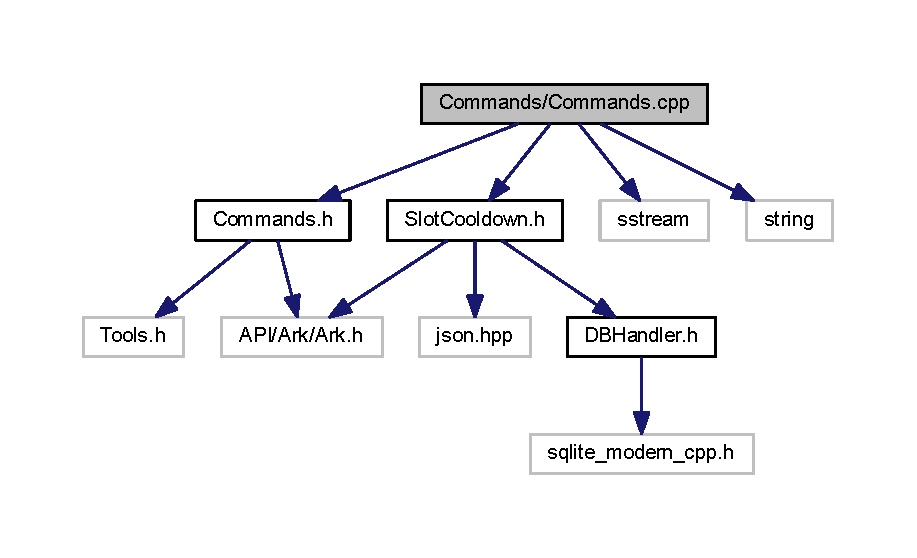
\includegraphics[width=350pt]{_commands_8cpp__incl}
\end{center}
\end{figure}
\subsection*{Classes}
\begin{DoxyCompactItemize}
\item 
struct \mbox{\hyperlink{struct_commands_1_1_slot_cooldown__t}{Commands\+::\+Slot\+Cooldown\+\_\+t}}
\begin{DoxyCompactList}\small\item\em time struct \end{DoxyCompactList}\end{DoxyCompactItemize}
\subsection*{Namespaces}
\begin{DoxyCompactItemize}
\item 
 \mbox{\hyperlink{namespace_commands}{Commands}}
\end{DoxyCompactItemize}
\subsection*{Functions}
\begin{DoxyCompactItemize}
\item 
void \mbox{\hyperlink{namespace_commands_a51cb85ec2c0f776aa53dcb6c8c2c7cd3}{Commands\+::\+Init\+Commands}} (void)
\begin{DoxyCompactList}\small\item\em Initialisation of commands. \end{DoxyCompactList}\item 
void \mbox{\hyperlink{namespace_commands_ae6511be8bafb608ff2b1861a98e3e4e6}{Commands\+::\+Remove\+Comands}} (void)
\begin{DoxyCompactList}\small\item\em Remove of commands. \end{DoxyCompactList}\end{DoxyCompactItemize}


\subsection{Detailed Description}
Implementation of all \mbox{\hyperlink{namespace_commands}{Commands}}. 

\begin{DoxyAuthor}{Author}
Matthias Birnthaler 
\end{DoxyAuthor}
\begin{DoxyDate}{Date}
15 May 2019 
\end{DoxyDate}

\hypertarget{_commands_8h}{}\section{Commands/\+Commands.h File Reference}
\label{_commands_8h}\index{Commands/\+Commands.\+h@{Commands/\+Commands.\+h}}


Implementation of all \mbox{\hyperlink{namespace_commands}{Commands}}.  


{\ttfamily \#include $<$A\+P\+I/\+Ark/\+Ark.\+h$>$}\newline
{\ttfamily \#include \char`\"{}Tools.\+h\char`\"{}}\newline
Include dependency graph for Commands.\+h\+:
\nopagebreak
\begin{figure}[H]
\begin{center}
\leavevmode
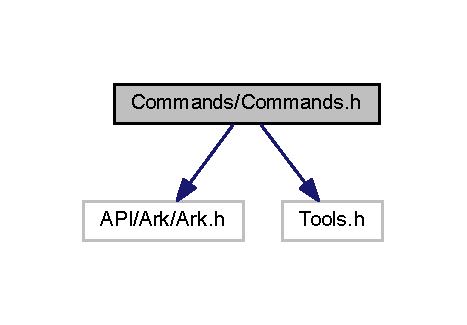
\includegraphics[width=224pt]{_commands_8h__incl}
\end{center}
\end{figure}
This graph shows which files directly or indirectly include this file\+:
\nopagebreak
\begin{figure}[H]
\begin{center}
\leavevmode
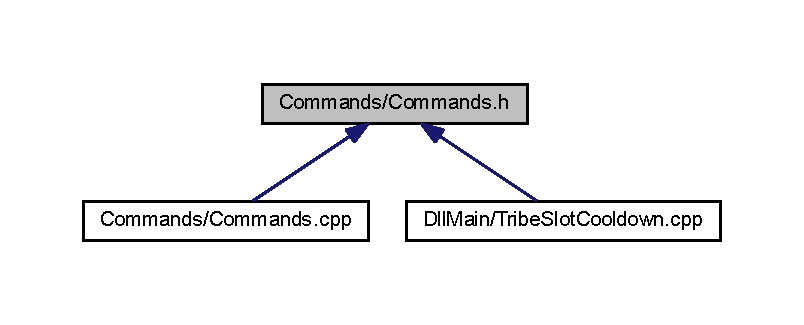
\includegraphics[width=350pt]{_commands_8h__dep__incl}
\end{center}
\end{figure}
\subsection*{Namespaces}
\begin{DoxyCompactItemize}
\item 
 \mbox{\hyperlink{namespace_commands}{Commands}}
\end{DoxyCompactItemize}
\subsection*{Functions}
\begin{DoxyCompactItemize}
\item 
void \mbox{\hyperlink{namespace_commands_a51cb85ec2c0f776aa53dcb6c8c2c7cd3}{Commands\+::\+Init\+Commands}} (void)
\begin{DoxyCompactList}\small\item\em Initialisation of commands. \end{DoxyCompactList}\item 
void \mbox{\hyperlink{namespace_commands_ae6511be8bafb608ff2b1861a98e3e4e6}{Commands\+::\+Remove\+Comands}} (void)
\begin{DoxyCompactList}\small\item\em Remove of commands. \end{DoxyCompactList}\end{DoxyCompactItemize}


\subsection{Detailed Description}
Implementation of all \mbox{\hyperlink{namespace_commands}{Commands}}. 

\begin{DoxyAuthor}{Author}
Matthias Birnthaler 
\end{DoxyAuthor}
\begin{DoxyDate}{Date}
15 May 2019 
\end{DoxyDate}

\hypertarget{_d_b_handler_8cpp}{}\section{D\+B\+Handler/\+D\+B\+Handler.cpp File Reference}
\label{_d_b_handler_8cpp}\index{D\+B\+Handler/\+D\+B\+Handler.\+cpp@{D\+B\+Handler/\+D\+B\+Handler.\+cpp}}


Interface to the database.  


{\ttfamily \#include \char`\"{}D\+B\+Handler.\+h\char`\"{}}\newline
{\ttfamily \#include \char`\"{}A\+P\+I/\+A\+R\+K/\+Ark.\+h\char`\"{}}\newline
Include dependency graph for D\+B\+Handler.\+cpp\+:
\nopagebreak
\begin{figure}[H]
\begin{center}
\leavevmode
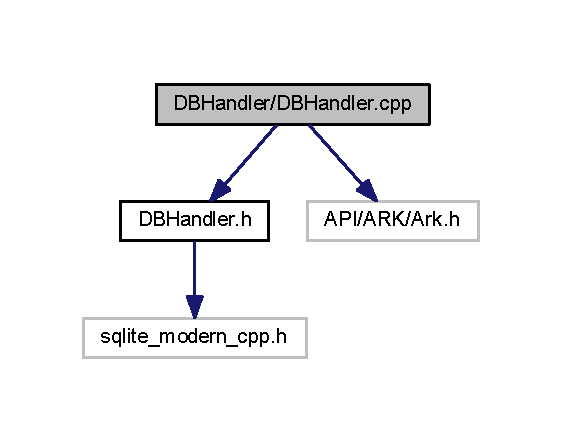
\includegraphics[width=270pt]{_d_b_handler_8cpp__incl}
\end{center}
\end{figure}


\subsection{Detailed Description}
Interface to the database. 

\begin{DoxyAuthor}{Author}
Matthias Birnthaler 
\end{DoxyAuthor}
\begin{DoxyDate}{Date}
15 May 2019 
\end{DoxyDate}

\hypertarget{_d_b_handler_8h}{}\section{D\+B\+Handler/\+D\+B\+Handler.h File Reference}
\label{_d_b_handler_8h}\index{D\+B\+Handler/\+D\+B\+Handler.\+h@{D\+B\+Handler/\+D\+B\+Handler.\+h}}


Interface to the database.  


{\ttfamily \#include $<$sqlite\+\_\+modern\+\_\+cpp.\+h$>$}\newline
Include dependency graph for D\+B\+Handler.\+h\+:
\nopagebreak
\begin{figure}[H]
\begin{center}
\leavevmode
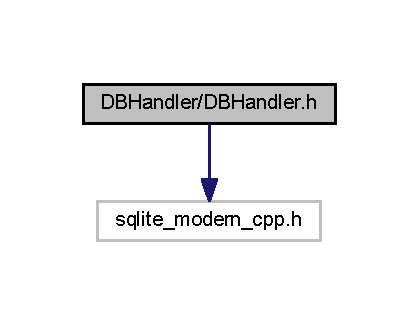
\includegraphics[width=201pt]{_d_b_handler_8h__incl}
\end{center}
\end{figure}
This graph shows which files directly or indirectly include this file\+:
\nopagebreak
\begin{figure}[H]
\begin{center}
\leavevmode
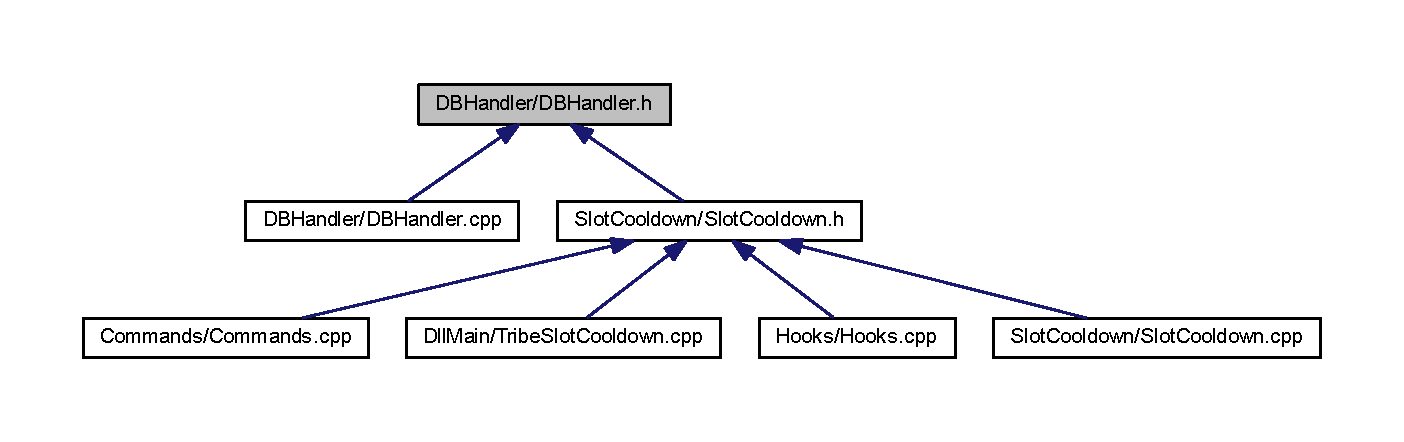
\includegraphics[width=350pt]{_d_b_handler_8h__dep__incl}
\end{center}
\end{figure}
\subsection*{Classes}
\begin{DoxyCompactItemize}
\item 
class \mbox{\hyperlink{class_d_b_handler}{D\+B\+Handler}}
\end{DoxyCompactItemize}


\subsection{Detailed Description}
Interface to the database. 

\begin{DoxyAuthor}{Author}
Matthias Birnthaler 
\end{DoxyAuthor}
\begin{DoxyDate}{Date}
15 May 2019 
\end{DoxyDate}

\hypertarget{_tribe_slot_cooldown_8cpp}{}\section{Dll\+Main/\+Tribe\+Slot\+Cooldown.cpp File Reference}
\label{_tribe_slot_cooldown_8cpp}\index{Dll\+Main/\+Tribe\+Slot\+Cooldown.\+cpp@{Dll\+Main/\+Tribe\+Slot\+Cooldown.\+cpp}}


Implementation of D\+L\+L\+Main.  


{\ttfamily \#include \char`\"{}Tribe\+Slot\+Cooldown.\+h\char`\"{}}\newline
{\ttfamily \#include \char`\"{}Slot\+Cooldown.\+h\char`\"{}}\newline
{\ttfamily \#include \char`\"{}Commands.\+h\char`\"{}}\newline
Include dependency graph for Tribe\+Slot\+Cooldown.\+cpp\+:
\nopagebreak
\begin{figure}[H]
\begin{center}
\leavevmode
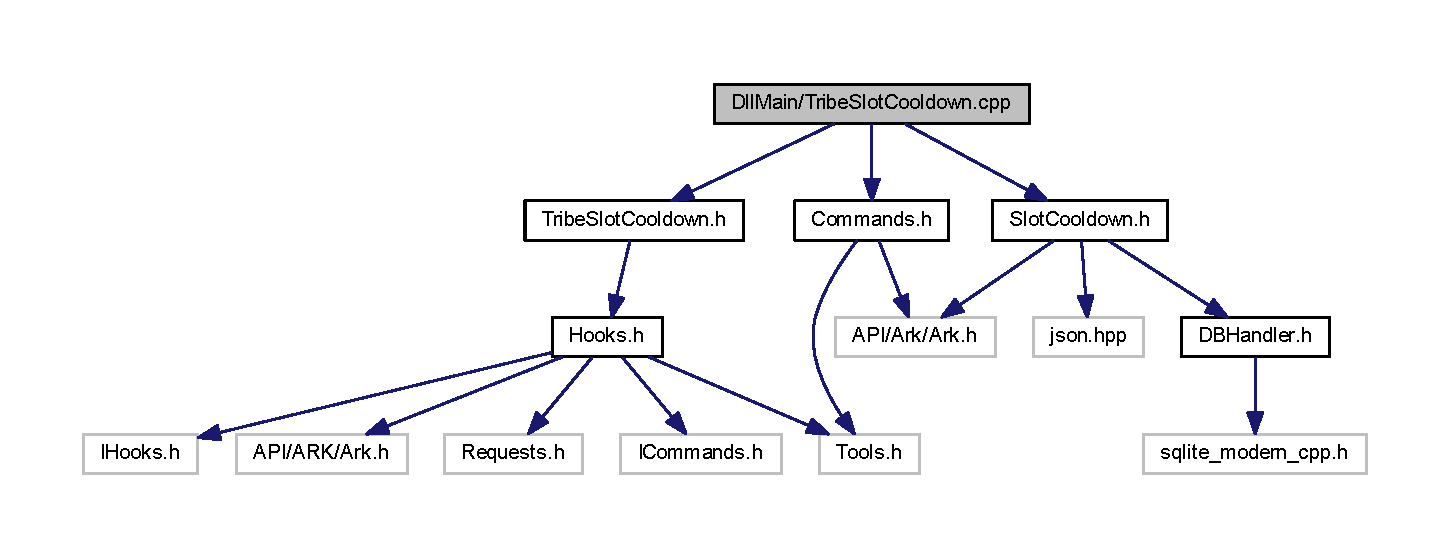
\includegraphics[width=350pt]{_tribe_slot_cooldown_8cpp__incl}
\end{center}
\end{figure}
\subsection*{Functions}
\begin{DoxyCompactItemize}
\item 
B\+O\+OL A\+P\+I\+E\+N\+T\+RY \mbox{\hyperlink{_tribe_slot_cooldown_8cpp_a26e64fb39b69bcd9d1274d279f1561b9}{Dll\+Main}} (H\+M\+O\+D\+U\+LE h\+Module, D\+W\+O\+RD ul\+\_\+reason\+\_\+for\+\_\+call, L\+P\+V\+O\+ID lp\+Reserved)
\begin{DoxyCompactList}\small\item\em D\+L\+L\+Main of the Tribe\+Slot\+Cooldown Plugin. \end{DoxyCompactList}\end{DoxyCompactItemize}


\subsection{Detailed Description}
Implementation of D\+L\+L\+Main. 

\begin{DoxyAuthor}{Author}
Matthias Birnthaler 
\end{DoxyAuthor}
\begin{DoxyDate}{Date}
15 May 2019 
\end{DoxyDate}


\subsection{Function Documentation}
\mbox{\Hypertarget{_tribe_slot_cooldown_8cpp_a26e64fb39b69bcd9d1274d279f1561b9}\label{_tribe_slot_cooldown_8cpp_a26e64fb39b69bcd9d1274d279f1561b9}} 
\index{Tribe\+Slot\+Cooldown.\+cpp@{Tribe\+Slot\+Cooldown.\+cpp}!Dll\+Main@{Dll\+Main}}
\index{Dll\+Main@{Dll\+Main}!Tribe\+Slot\+Cooldown.\+cpp@{Tribe\+Slot\+Cooldown.\+cpp}}
\subsubsection{\texorpdfstring{Dll\+Main()}{DllMain()}}
{\footnotesize\ttfamily B\+O\+OL A\+P\+I\+E\+N\+T\+RY Dll\+Main (\begin{DoxyParamCaption}\item[{H\+M\+O\+D\+U\+LE}]{h\+Module,  }\item[{D\+W\+O\+RD}]{ul\+\_\+reason\+\_\+for\+\_\+call,  }\item[{L\+P\+V\+O\+ID}]{lp\+Reserved }\end{DoxyParamCaption})}



D\+L\+L\+Main of the Tribe\+Slot\+Cooldown Plugin. 


\begin{DoxyParams}[1]{Parameters}
\mbox{\tt in}  & {\em h\+Module} & \\
\hline
\mbox{\tt in}  & {\em ul\+\_\+reason\+\_\+for\+\_\+call} & \\
\hline
\mbox{\tt in}  & {\em lp\+Reserved} & \\
\hline
\end{DoxyParams}
\begin{DoxyReturn}{Returns}
B\+O\+OL 
\end{DoxyReturn}

\hypertarget{_tribe_slot_cooldown_8h}{}\section{Dll\+Main/\+Tribe\+Slot\+Cooldown.h File Reference}
\label{_tribe_slot_cooldown_8h}\index{Dll\+Main/\+Tribe\+Slot\+Cooldown.\+h@{Dll\+Main/\+Tribe\+Slot\+Cooldown.\+h}}


Implementation of D\+L\+L\+Main.  


{\ttfamily \#include \char`\"{}Hooks.\+h\char`\"{}}\newline
Include dependency graph for Tribe\+Slot\+Cooldown.\+h\+:
\nopagebreak
\begin{figure}[H]
\begin{center}
\leavevmode
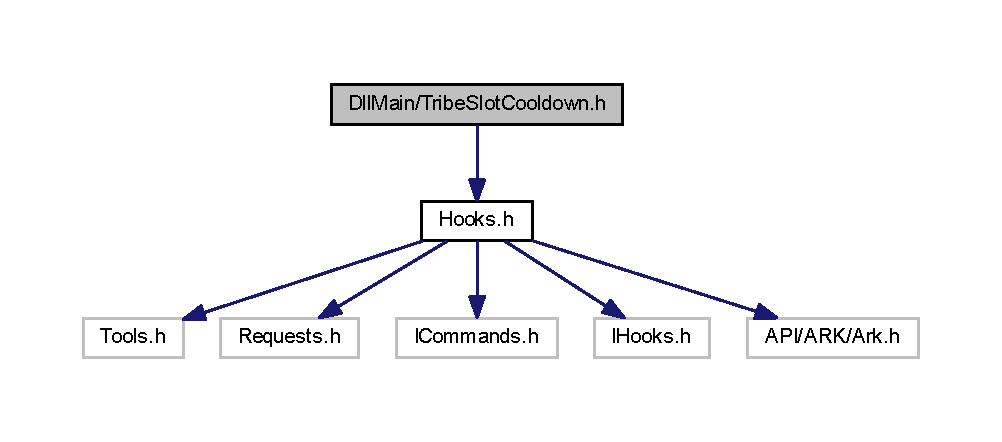
\includegraphics[width=350pt]{_tribe_slot_cooldown_8h__incl}
\end{center}
\end{figure}
This graph shows which files directly or indirectly include this file\+:
\nopagebreak
\begin{figure}[H]
\begin{center}
\leavevmode
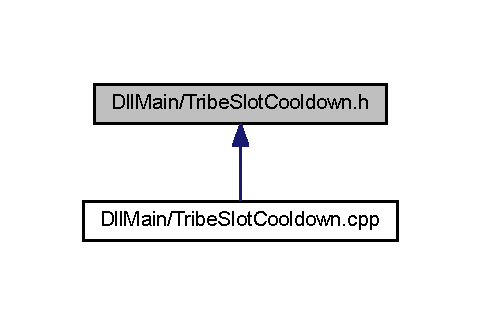
\includegraphics[width=231pt]{_tribe_slot_cooldown_8h__dep__incl}
\end{center}
\end{figure}
\subsection*{Functions}
\begin{DoxyCompactItemize}
\item 
B\+O\+OL A\+P\+I\+E\+N\+T\+RY \mbox{\hyperlink{_tribe_slot_cooldown_8h_a26e64fb39b69bcd9d1274d279f1561b9}{Dll\+Main}} (H\+M\+O\+D\+U\+LE h\+Module, D\+W\+O\+RD ul\+\_\+reason\+\_\+for\+\_\+call, L\+P\+V\+O\+ID lp\+Reserved)
\begin{DoxyCompactList}\small\item\em D\+L\+L\+Main of the Tribe\+Slot\+Cooldown Plugin. \end{DoxyCompactList}\end{DoxyCompactItemize}


\subsection{Detailed Description}
Implementation of D\+L\+L\+Main. 

\begin{DoxyAuthor}{Author}
Matthias Birnthaler 
\end{DoxyAuthor}
\begin{DoxyDate}{Date}
15 May 2019 
\end{DoxyDate}


\subsection{Function Documentation}
\mbox{\Hypertarget{_tribe_slot_cooldown_8h_a26e64fb39b69bcd9d1274d279f1561b9}\label{_tribe_slot_cooldown_8h_a26e64fb39b69bcd9d1274d279f1561b9}} 
\index{Tribe\+Slot\+Cooldown.\+h@{Tribe\+Slot\+Cooldown.\+h}!Dll\+Main@{Dll\+Main}}
\index{Dll\+Main@{Dll\+Main}!Tribe\+Slot\+Cooldown.\+h@{Tribe\+Slot\+Cooldown.\+h}}
\subsubsection{\texorpdfstring{Dll\+Main()}{DllMain()}}
{\footnotesize\ttfamily B\+O\+OL A\+P\+I\+E\+N\+T\+RY Dll\+Main (\begin{DoxyParamCaption}\item[{H\+M\+O\+D\+U\+LE}]{h\+Module,  }\item[{D\+W\+O\+RD}]{ul\+\_\+reason\+\_\+for\+\_\+call,  }\item[{L\+P\+V\+O\+ID}]{lp\+Reserved }\end{DoxyParamCaption})}



D\+L\+L\+Main of the Tribe\+Slot\+Cooldown Plugin. 


\begin{DoxyParams}[1]{Parameters}
\mbox{\tt in}  & {\em h\+Module} & \\
\hline
\mbox{\tt in}  & {\em ul\+\_\+reason\+\_\+for\+\_\+call} & \\
\hline
\mbox{\tt in}  & {\em lp\+Reserved} & \\
\hline
\end{DoxyParams}
\begin{DoxyReturn}{Returns}
B\+O\+OL 
\end{DoxyReturn}

\hypertarget{_hooks_8cpp}{}\section{Hooks/\+Hooks.cpp File Reference}
\label{_hooks_8cpp}\index{Hooks/\+Hooks.\+cpp@{Hooks/\+Hooks.\+cpp}}


File containing the implementation for all needed Hooks.  


{\ttfamily \#include \char`\"{}Hooks.\+h\char`\"{}}\newline
{\ttfamily \#include \char`\"{}Slot\+Cooldown.\+h\char`\"{}}\newline
Include dependency graph for Hooks.\+cpp\+:
\nopagebreak
\begin{figure}[H]
\begin{center}
\leavevmode
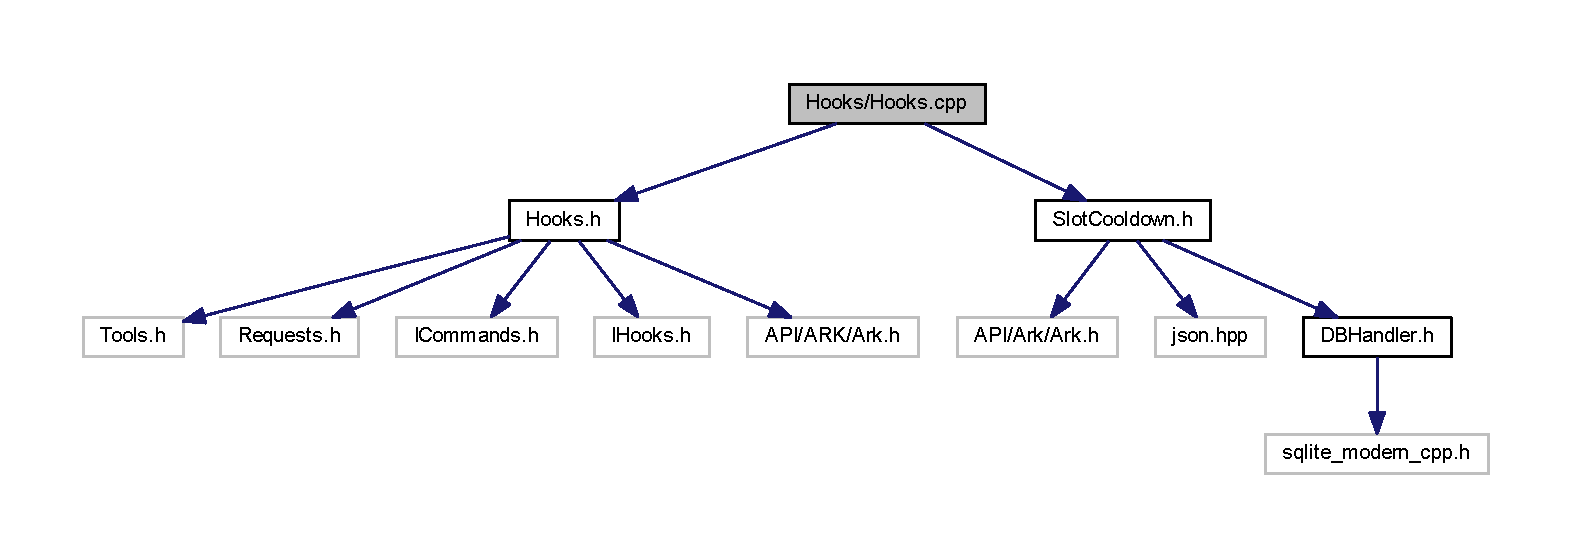
\includegraphics[width=350pt]{_hooks_8cpp__incl}
\end{center}
\end{figure}
\subsection*{Functions}
\begin{DoxyCompactItemize}
\item 
void \mbox{\hyperlink{_hooks_8cpp_a3d35c0782ddf529d074136c74e16703c}{Init\+Hooks}} (void)
\begin{DoxyCompactList}\small\item\em Initialisation of needed Hooks. \end{DoxyCompactList}\item 
void \mbox{\hyperlink{_hooks_8cpp_a37fd3027b8b64aad7f198e4a6272a2f8}{Remove\+Hooks}} (void)
\begin{DoxyCompactList}\small\item\em Cancellation of needed Hooks. \end{DoxyCompactList}\end{DoxyCompactItemize}


\subsection{Detailed Description}
File containing the implementation for all needed Hooks. 

\begin{DoxyAuthor}{Author}
Matthias Birnthaler 
\end{DoxyAuthor}
\begin{DoxyDate}{Date}
15 May 2019 
\end{DoxyDate}


\subsection{Function Documentation}
\mbox{\Hypertarget{_hooks_8cpp_a3d35c0782ddf529d074136c74e16703c}\label{_hooks_8cpp_a3d35c0782ddf529d074136c74e16703c}} 
\index{Hooks.\+cpp@{Hooks.\+cpp}!Init\+Hooks@{Init\+Hooks}}
\index{Init\+Hooks@{Init\+Hooks}!Hooks.\+cpp@{Hooks.\+cpp}}
\subsubsection{\texorpdfstring{Init\+Hooks()}{InitHooks()}}
{\footnotesize\ttfamily void Init\+Hooks (\begin{DoxyParamCaption}\item[{void}]{ }\end{DoxyParamCaption})}



Initialisation of needed Hooks. 

This function initialise all needed Hooks

\begin{DoxyReturn}{Returns}
void 
\end{DoxyReturn}
\mbox{\Hypertarget{_hooks_8cpp_a37fd3027b8b64aad7f198e4a6272a2f8}\label{_hooks_8cpp_a37fd3027b8b64aad7f198e4a6272a2f8}} 
\index{Hooks.\+cpp@{Hooks.\+cpp}!Remove\+Hooks@{Remove\+Hooks}}
\index{Remove\+Hooks@{Remove\+Hooks}!Hooks.\+cpp@{Hooks.\+cpp}}
\subsubsection{\texorpdfstring{Remove\+Hooks()}{RemoveHooks()}}
{\footnotesize\ttfamily void Remove\+Hooks (\begin{DoxyParamCaption}\item[{void}]{ }\end{DoxyParamCaption})}



Cancellation of needed Hooks. 

This function removes all needed Hooks.

\begin{DoxyReturn}{Returns}
void 
\end{DoxyReturn}

\hypertarget{_hooks_8h}{}\section{Hooks/\+Hooks.h File Reference}
\label{_hooks_8h}\index{Hooks/\+Hooks.\+h@{Hooks/\+Hooks.\+h}}


File containing the implementation for all needed Hooks.  


{\ttfamily \#include \char`\"{}Tools.\+h\char`\"{}}\newline
{\ttfamily \#include \char`\"{}Requests.\+h\char`\"{}}\newline
{\ttfamily \#include \char`\"{}I\+Commands.\+h\char`\"{}}\newline
{\ttfamily \#include \char`\"{}I\+Hooks.\+h\char`\"{}}\newline
{\ttfamily \#include \char`\"{}A\+P\+I/\+A\+R\+K/\+Ark.\+h\char`\"{}}\newline
Include dependency graph for Hooks.\+h\+:
\nopagebreak
\begin{figure}[H]
\begin{center}
\leavevmode
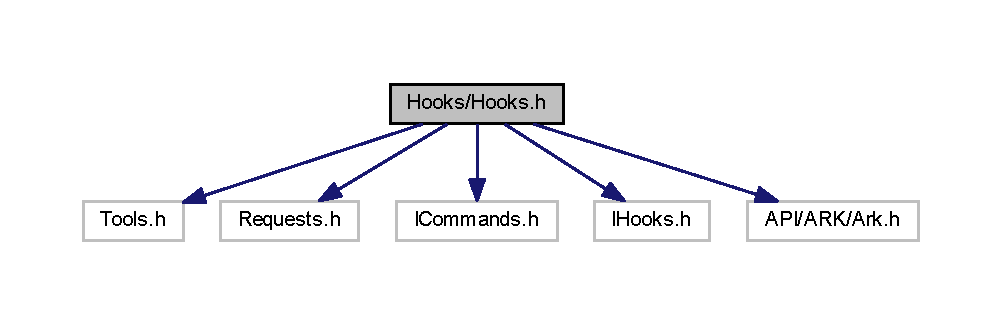
\includegraphics[width=350pt]{_hooks_8h__incl}
\end{center}
\end{figure}
This graph shows which files directly or indirectly include this file\+:
\nopagebreak
\begin{figure}[H]
\begin{center}
\leavevmode
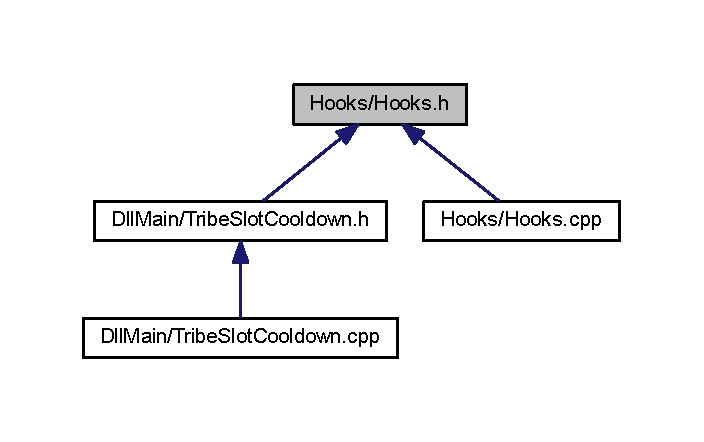
\includegraphics[width=338pt]{_hooks_8h__dep__incl}
\end{center}
\end{figure}
\subsection*{Functions}
\begin{DoxyCompactItemize}
\item 
\mbox{\hyperlink{_hooks_8h_a1dea30ea2d347da31e3339a1f72ab830}{D\+E\+C\+L\+A\+R\+E\+\_\+\+H\+O\+OK}} (A\+Shooter\+Player\+State\+\_\+\+Add\+To\+Tribe, bool, A\+Shooter\+Player\+State $\ast$, F\+Tribe\+Data $\ast$, bool, bool, bool, A\+Player\+Controller $\ast$)
\begin{DoxyCompactList}\small\item\em declare of A\+Shooter\+Player\+State\+\_\+\+Add\+To\+Tribe Hook \end{DoxyCompactList}\item 
\mbox{\hyperlink{_hooks_8h_adae8ecd506a04eca9e4229161e89a26c}{D\+E\+C\+L\+A\+R\+E\+\_\+\+H\+O\+OK}} (A\+Shooter\+Game\+Mode\+\_\+\+Remove\+Player\+From\+Tribe, void, A\+Shooter\+Game\+Mode $\ast$, unsigned \+\_\+\+\_\+int64, unsigned \+\_\+\+\_\+int64, bool)
\item 
void \mbox{\hyperlink{_hooks_8h_a3d35c0782ddf529d074136c74e16703c}{Init\+Hooks}} (void)
\begin{DoxyCompactList}\small\item\em Initialisation of needed Hooks. \end{DoxyCompactList}\item 
void \mbox{\hyperlink{_hooks_8h_a37fd3027b8b64aad7f198e4a6272a2f8}{Remove\+Hooks}} (void)
\begin{DoxyCompactList}\small\item\em Cancellation of needed Hooks. \end{DoxyCompactList}\end{DoxyCompactItemize}


\subsection{Detailed Description}
File containing the implementation for all needed Hooks. 

\begin{DoxyAuthor}{Author}
Matthias Birnthaler 
\end{DoxyAuthor}
\begin{DoxyDate}{Date}
15 May 2019 
\end{DoxyDate}


\subsection{Function Documentation}
\mbox{\Hypertarget{_hooks_8h_a1dea30ea2d347da31e3339a1f72ab830}\label{_hooks_8h_a1dea30ea2d347da31e3339a1f72ab830}} 
\index{Hooks.\+h@{Hooks.\+h}!D\+E\+C\+L\+A\+R\+E\+\_\+\+H\+O\+OK@{D\+E\+C\+L\+A\+R\+E\+\_\+\+H\+O\+OK}}
\index{D\+E\+C\+L\+A\+R\+E\+\_\+\+H\+O\+OK@{D\+E\+C\+L\+A\+R\+E\+\_\+\+H\+O\+OK}!Hooks.\+h@{Hooks.\+h}}
\subsubsection{\texorpdfstring{D\+E\+C\+L\+A\+R\+E\+\_\+\+H\+O\+O\+K()}{DECLARE\_HOOK()}\hspace{0.1cm}{\footnotesize\ttfamily [1/2]}}
{\footnotesize\ttfamily D\+E\+C\+L\+A\+R\+E\+\_\+\+H\+O\+OK (\begin{DoxyParamCaption}\item[{A\+Shooter\+Player\+State\+\_\+\+Add\+To\+Tribe}]{,  }\item[{bool}]{,  }\item[{A\+Shooter\+Player\+State $\ast$}]{,  }\item[{F\+Tribe\+Data $\ast$}]{,  }\item[{bool}]{,  }\item[{bool}]{,  }\item[{bool}]{,  }\item[{A\+Player\+Controller $\ast$}]{ }\end{DoxyParamCaption})}



declare of A\+Shooter\+Player\+State\+\_\+\+Add\+To\+Tribe Hook 

$<$declare of A\+Shooter\+Game\+Mode\+\_\+\+Remove\+Player\+From\+Tribe Hook \mbox{\Hypertarget{_hooks_8h_adae8ecd506a04eca9e4229161e89a26c}\label{_hooks_8h_adae8ecd506a04eca9e4229161e89a26c}} 
\index{Hooks.\+h@{Hooks.\+h}!D\+E\+C\+L\+A\+R\+E\+\_\+\+H\+O\+OK@{D\+E\+C\+L\+A\+R\+E\+\_\+\+H\+O\+OK}}
\index{D\+E\+C\+L\+A\+R\+E\+\_\+\+H\+O\+OK@{D\+E\+C\+L\+A\+R\+E\+\_\+\+H\+O\+OK}!Hooks.\+h@{Hooks.\+h}}
\subsubsection{\texorpdfstring{D\+E\+C\+L\+A\+R\+E\+\_\+\+H\+O\+O\+K()}{DECLARE\_HOOK()}\hspace{0.1cm}{\footnotesize\ttfamily [2/2]}}
{\footnotesize\ttfamily D\+E\+C\+L\+A\+R\+E\+\_\+\+H\+O\+OK (\begin{DoxyParamCaption}\item[{A\+Shooter\+Game\+Mode\+\_\+\+Remove\+Player\+From\+Tribe}]{,  }\item[{void}]{,  }\item[{A\+Shooter\+Game\+Mode $\ast$}]{,  }\item[{unsigned}]{\+\_\+\+\_\+int64,  }\item[{unsigned}]{\+\_\+\+\_\+int64,  }\item[{bool}]{ }\end{DoxyParamCaption})}

\mbox{\Hypertarget{_hooks_8h_a3d35c0782ddf529d074136c74e16703c}\label{_hooks_8h_a3d35c0782ddf529d074136c74e16703c}} 
\index{Hooks.\+h@{Hooks.\+h}!Init\+Hooks@{Init\+Hooks}}
\index{Init\+Hooks@{Init\+Hooks}!Hooks.\+h@{Hooks.\+h}}
\subsubsection{\texorpdfstring{Init\+Hooks()}{InitHooks()}}
{\footnotesize\ttfamily void Init\+Hooks (\begin{DoxyParamCaption}\item[{void}]{ }\end{DoxyParamCaption})}



Initialisation of needed Hooks. 

This function initialise all needed Hooks

\begin{DoxyReturn}{Returns}
void 
\end{DoxyReturn}
\mbox{\Hypertarget{_hooks_8h_a37fd3027b8b64aad7f198e4a6272a2f8}\label{_hooks_8h_a37fd3027b8b64aad7f198e4a6272a2f8}} 
\index{Hooks.\+h@{Hooks.\+h}!Remove\+Hooks@{Remove\+Hooks}}
\index{Remove\+Hooks@{Remove\+Hooks}!Hooks.\+h@{Hooks.\+h}}
\subsubsection{\texorpdfstring{Remove\+Hooks()}{RemoveHooks()}}
{\footnotesize\ttfamily void Remove\+Hooks (\begin{DoxyParamCaption}\item[{void}]{ }\end{DoxyParamCaption})}



Cancellation of needed Hooks. 

This function removes all needed Hooks.

\begin{DoxyReturn}{Returns}
void 
\end{DoxyReturn}

\hypertarget{_slot_cooldown_8cpp}{}\section{Slot\+Cooldown/\+Slot\+Cooldown.cpp File Reference}
\label{_slot_cooldown_8cpp}\index{Slot\+Cooldown/\+Slot\+Cooldown.\+cpp@{Slot\+Cooldown/\+Slot\+Cooldown.\+cpp}}


Implementation of the player slots cooldown logic.  


{\ttfamily \#include \char`\"{}Slot\+Cooldown.\+h\char`\"{}}\newline
{\ttfamily \#include $<$fstream$>$}\newline
Include dependency graph for Slot\+Cooldown.\+cpp\+:
\nopagebreak
\begin{figure}[H]
\begin{center}
\leavevmode
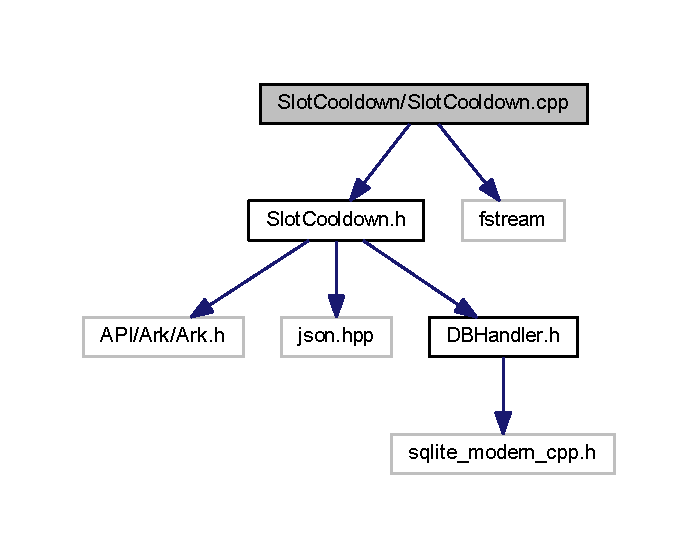
\includegraphics[width=335pt]{_slot_cooldown_8cpp__incl}
\end{center}
\end{figure}
\subsection*{Namespaces}
\begin{DoxyCompactItemize}
\item 
 \mbox{\hyperlink{namespace_slot_cooldown}{Slot\+Cooldown}}
\end{DoxyCompactItemize}
\subsection*{Functions}
\begin{DoxyCompactItemize}
\item 
void \mbox{\hyperlink{namespace_slot_cooldown_af1d102851d318b69e6b808f8c1b0f6fa}{Slot\+Cooldown\+::\+Init\+Slot\+Cooldown}} (void)
\begin{DoxyCompactList}\small\item\em Initialisation of the Slot Cooldown. \end{DoxyCompactList}\item 
void \mbox{\hyperlink{namespace_slot_cooldown_acadf0d52f01444ce96d02fefd725abe8}{Slot\+Cooldown\+::\+Normalize\+Slots}} (std\+::vector$<$ int $>$ $\ast$slots, long double Server\+Run\+Time)
\begin{DoxyCompactList}\small\item\em Normalize slot cooldowns. \end{DoxyCompactList}\item 
void \mbox{\hyperlink{namespace_slot_cooldown_ad36d7fcdac6fac169b44ce05b3ea98f9}{Slot\+Cooldown\+::\+Set\+Tribe\+Slot\+To\+Cooldown}} (int Tribe\+Id)
\begin{DoxyCompactList}\small\item\em Sets tribe slot to cooldown. \end{DoxyCompactList}\item 
bool \mbox{\hyperlink{namespace_slot_cooldown_af34a0fce4996c0cb1f108dea38c9c00c}{Slot\+Cooldown\+::\+Suppress\+Player\+Join\+Tribe}} (int Tribe\+Id, int Players\+In\+Tribe)
\begin{DoxyCompactList}\small\item\em Checks if it is possible to join a tribe. \end{DoxyCompactList}\item 
bool \mbox{\hyperlink{namespace_slot_cooldown_aa61b482a7729c7eb2a23d068f74477c3}{Slot\+Cooldown\+::\+Suppress\+Tribe\+Merge}} (int Tribe\+Id\+New\+Tribe, int Tribe\+Id\+Old\+Tribe, int Num\+Players\+In\+New\+Tribe, int Num\+Players\+In\+Old\+Tribe)
\begin{DoxyCompactList}\small\item\em Checks if it is possible to merge a tribe. \end{DoxyCompactList}\end{DoxyCompactItemize}
\subsection*{Variables}
\begin{DoxyCompactItemize}
\item 
F\+String \mbox{\hyperlink{namespace_slot_cooldown_ad9b4de67b82bb1e9f21fd5d5674b34be}{Slot\+Cooldown\+::\+Suppress\+Player\+Join\+Tribe\+Message}}
\begin{DoxyCompactList}\small\item\em Message for the player if tribe join is not possible. \end{DoxyCompactList}\item 
F\+String \mbox{\hyperlink{namespace_slot_cooldown_abd12b2304b5bf308744798daca9419f6}{Slot\+Cooldown\+::\+Suppress\+Merge\+Tribe\+Message}}
\begin{DoxyCompactList}\small\item\em Message for the player if tribe merge is not possible. \end{DoxyCompactList}\item 
F\+String \mbox{\hyperlink{namespace_slot_cooldown_a96c0601961d6636388621ee070136bd8}{Slot\+Cooldown\+::\+Command\+Display\+Slots\+Message}}
\begin{DoxyCompactList}\small\item\em Message for the player with the total of tribe player slots with cooldown. \end{DoxyCompactList}\item 
F\+String \mbox{\hyperlink{namespace_slot_cooldown_ac0a5c9ed81d34ecf571126bc0ce8e1e7}{Slot\+Cooldown\+::\+Command\+Display\+Slots\+Message\+Slot\+Cooldown}}
\begin{DoxyCompactList}\small\item\em Message for the player with the left time for a slots cooldown. \end{DoxyCompactList}\item 
F\+String \mbox{\hyperlink{namespace_slot_cooldown_a5b94faf2e06664e82c8811880e3ac662}{Slot\+Cooldown\+::\+Command\+Prefix}}
\begin{DoxyCompactList}\small\item\em Prefix for chat commands. \end{DoxyCompactList}\item 
F\+String \mbox{\hyperlink{namespace_slot_cooldown_a5785ecad34ad6558721c26503620eeb2}{Slot\+Cooldown\+::\+Command\+Display\+Slots}}
\begin{DoxyCompactList}\small\item\em String for chat command display slots with cooldown. \end{DoxyCompactList}\item 
float \mbox{\hyperlink{namespace_slot_cooldown_a45d147dcd56cfa641b7dc9f9303db683}{Slot\+Cooldown\+::\+Message\+Display\+Size}}
\begin{DoxyCompactList}\small\item\em Size of player notifications. \end{DoxyCompactList}\item 
float \mbox{\hyperlink{namespace_slot_cooldown_a9c1b0776e8b6e909e5a94f465c7669e1}{Slot\+Cooldown\+::\+Message\+Display\+Time}}
\begin{DoxyCompactList}\small\item\em Display time for player notifications. \end{DoxyCompactList}\item 
float \mbox{\hyperlink{namespace_slot_cooldown_a1684ab6db297facc86efbca540cd19f9}{Slot\+Cooldown\+::\+Slot\+Cooldown}}
\begin{DoxyCompactList}\small\item\em Cooldown time for slots in secounds. \end{DoxyCompactList}\end{DoxyCompactItemize}


\subsection{Detailed Description}
Implementation of the player slots cooldown logic. 

\begin{DoxyAuthor}{Author}
Matthias Birnthaler 
\end{DoxyAuthor}
\begin{DoxyDate}{Date}
15 May 2019 
\end{DoxyDate}

\hypertarget{_slot_cooldown_8h}{}\section{Slot\+Cooldown/\+Slot\+Cooldown.h File Reference}
\label{_slot_cooldown_8h}\index{Slot\+Cooldown/\+Slot\+Cooldown.\+h@{Slot\+Cooldown/\+Slot\+Cooldown.\+h}}


Implementation of the player slots cooldown logic.  


{\ttfamily \#include $<$A\+P\+I/\+Ark/\+Ark.\+h$>$}\newline
{\ttfamily \#include \char`\"{}json.\+hpp\char`\"{}}\newline
{\ttfamily \#include \char`\"{}D\+B\+Handler.\+h\char`\"{}}\newline
Include dependency graph for Slot\+Cooldown.\+h\+:
\nopagebreak
\begin{figure}[H]
\begin{center}
\leavevmode
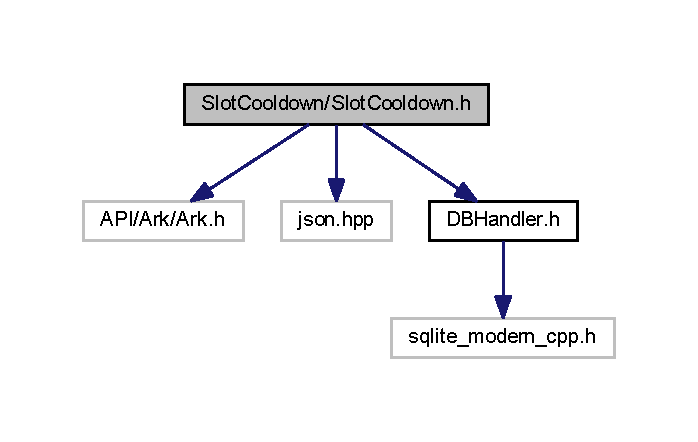
\includegraphics[width=335pt]{_slot_cooldown_8h__incl}
\end{center}
\end{figure}
This graph shows which files directly or indirectly include this file\+:
\nopagebreak
\begin{figure}[H]
\begin{center}
\leavevmode
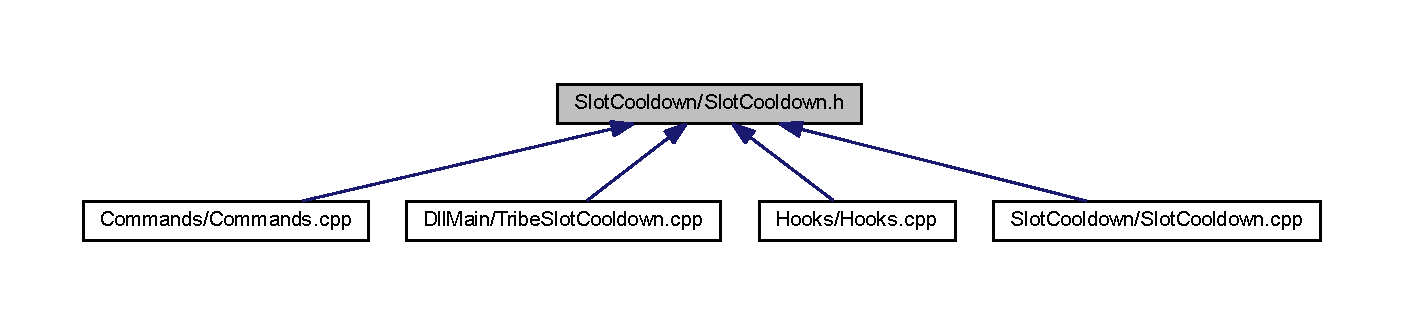
\includegraphics[width=350pt]{_slot_cooldown_8h__dep__incl}
\end{center}
\end{figure}
\subsection*{Namespaces}
\begin{DoxyCompactItemize}
\item 
 \mbox{\hyperlink{namespace_slot_cooldown}{Slot\+Cooldown}}
\end{DoxyCompactItemize}
\subsection*{Functions}
\begin{DoxyCompactItemize}
\item 
void \mbox{\hyperlink{namespace_slot_cooldown_af1d102851d318b69e6b808f8c1b0f6fa}{Slot\+Cooldown\+::\+Init\+Slot\+Cooldown}} (void)
\begin{DoxyCompactList}\small\item\em Initialisation of the Slot Cooldown. \end{DoxyCompactList}\item 
void \mbox{\hyperlink{namespace_slot_cooldown_acadf0d52f01444ce96d02fefd725abe8}{Slot\+Cooldown\+::\+Normalize\+Slots}} (std\+::vector$<$ int $>$ $\ast$slots, long double Server\+Run\+Time)
\begin{DoxyCompactList}\small\item\em Normalize slot cooldowns. \end{DoxyCompactList}\item 
void \mbox{\hyperlink{namespace_slot_cooldown_ad36d7fcdac6fac169b44ce05b3ea98f9}{Slot\+Cooldown\+::\+Set\+Tribe\+Slot\+To\+Cooldown}} (int Tribe\+Id)
\begin{DoxyCompactList}\small\item\em Sets tribe slot to cooldown. \end{DoxyCompactList}\item 
bool \mbox{\hyperlink{namespace_slot_cooldown_af34a0fce4996c0cb1f108dea38c9c00c}{Slot\+Cooldown\+::\+Suppress\+Player\+Join\+Tribe}} (int Tribe\+Id, int Players\+In\+Tribe)
\begin{DoxyCompactList}\small\item\em Checks if it is possible to join a tribe. \end{DoxyCompactList}\item 
bool \mbox{\hyperlink{namespace_slot_cooldown_aa61b482a7729c7eb2a23d068f74477c3}{Slot\+Cooldown\+::\+Suppress\+Tribe\+Merge}} (int Tribe\+Id\+New\+Tribe, int Tribe\+Id\+Old\+Tribe, int Num\+Players\+In\+New\+Tribe, int Num\+Players\+In\+Old\+Tribe)
\begin{DoxyCompactList}\small\item\em Checks if it is possible to merge a tribe. \end{DoxyCompactList}\end{DoxyCompactItemize}
\subsection*{Variables}
\begin{DoxyCompactItemize}
\item 
std\+::unique\+\_\+ptr$<$ \mbox{\hyperlink{class_d_b_handler}{D\+B\+Handler}} $>$ \mbox{\hyperlink{namespace_slot_cooldown_a0945ac0ffac4f4655877d61f50837c70}{Slot\+Cooldown\+::database}}
\begin{DoxyCompactList}\small\item\em Interface database. \end{DoxyCompactList}\end{DoxyCompactItemize}


\subsection{Detailed Description}
Implementation of the player slots cooldown logic. 

\begin{DoxyAuthor}{Author}
Matthias Birnthaler 
\end{DoxyAuthor}
\begin{DoxyDate}{Date}
15 May 2019 
\end{DoxyDate}

%--- End generated contents ---

% Index
\backmatter
\newpage
\phantomsection
\clearemptydoublepage
\addcontentsline{toc}{chapter}{Index}
\printindex

\end{document}
